% title: Trace, transform, execute
% description: Tracing records a Python function as IR. A transform returns another IR. Execution uses runtime inputs to produce an output.
\documentclass[tikz,border=5pt]{standalone}
\usetikzlibrary{arrows.meta,shapes.geometric}
\begin{document}
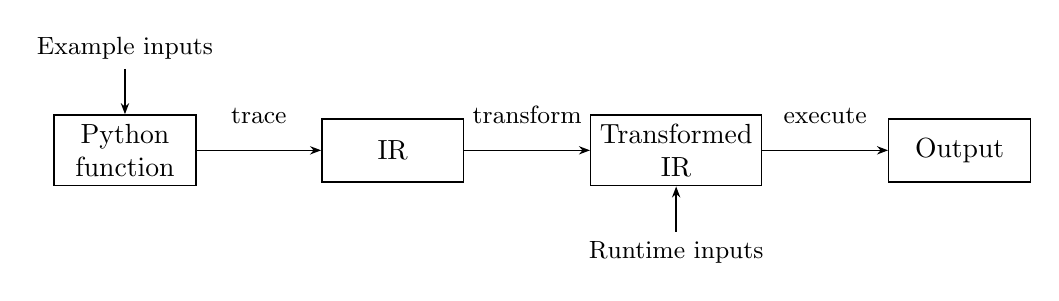
\begin{tikzpicture}[
    box/.style={draw, line width=0.5pt, minimum height=0.8cm,
                minimum width=1.8cm, align=center},
    flow/.style={-{Stealth[length=4pt]}, line width=0.5pt},
    note/.style={font=\small, align=center},
    choice/.style={diamond, draw, line width=0.5pt,
                   aspect=2, inner sep=2pt, align=center},
]

    \node[box] (function) at (0,0) {Python\\function};
    \node[box] (ir) at (3.4,0) {IR};
    \node[box] (new) at (7,0) {Transformed\\IR};
    \node[box] (output) at (10.6,0) {Output};
    \draw[flow] (function) -- node[above=6pt,note] {trace} (ir);
    \draw[flow] (ir) -- node[above=6pt,note] {transform} (new);
    \draw[flow] (new) -- node[above=6pt,note] {execute} (output);
    \node[note] (examples) at (0,1.3) {Example inputs};
    \draw[flow] (examples) -- (function);
    \node[note] (inputs) at (7,-1.3) {Runtime inputs};
    \draw[flow] (inputs) -- (new);

\end{tikzpicture}
\end{document}
